\begin{figure}
  \hspace*{20mm}
  \begin{tikzpicture}
    \node[inner sep=0pt] (circuit) at (0,0) {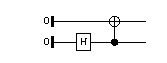
\includegraphics[scale=2]{Figures/circuits/Bell}};
    \node[right=8mm of circuit.north west, font=\itshape] (text) {a)};
  \end{tikzpicture} 
  \begin{tikzpicture}
    \node[inner sep=0pt] (circuit) at (0,0) {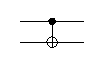
\includegraphics[scale=2, trim={5mm 0 0 0},clip]{Figures/circuits/CNOT}};
    \node[rectangle, fill=white, minimum size=5mm] (clear) at (-5mm,-5mm) {};
    \pic (e1) {ebit=e1/5.63mm/13mm};
    \node[right=2mm of circuit.north west, font=\itshape] (text) {b)};
  \end{tikzpicture}
\caption{Generation of the Bell state \(\ket{\Phi^+} = \frac{1}{\sqrt{2}}\ket{0,0} + \frac{1}{\sqrt{2}}\ket{1,1}\) shown in \textit{a)}. Its shorthand circuit notation is given in \textit{b)}.}
\label{fig:bell}
\end{figure}